\chapter{Introduction to Text Mining with Machine Learning}
\section{Introduction}

In the last few years, we have seen an explosion in the amount of data as the result of many activities.
The data comes from various sources and is available in many formats.
This has been enabled, primarily, by the massive advance on the Internet.
Various devices like smart phones enable communication and the use of applications anytime and anywhere;
many activities like shopping, interacting with government institutions, or providing support to customers, are moving to digital environments;
many documents are being digitalized; people meet and interact on virtual platforms.
The transformation of the Web into Web 2.0\cite{ref26}, where the content is actively created by users, has thrown open to the masses, many possible avenues to express their ideas, recommendations, or attitudes.

It is obvious that texts written in a natural language are a natural way of human communication.
Textual documents are thus strongly related to many human activities and they have become a source that is worth analyzing.
The results of such an analysis can bring useful insights in practically all domains.

As the ability of people to analyze texts remains essentially the same, the availability of more data requires new computational methods in order to find something useful in large collections of documents.
Thus, a discipline known as \textit{text mining} has become very popular and attractive.
Text mining can be defined as a knowledge-intensive process in which a user interacts with a collection of documents by using analytic tools in order to identify and explore interesting
patterns \cite{ref87}. Applications can be found in marketing, competitive intelligence,
banking, health care, manufacturing, security, natural sciences, and many other
domains \cite{ref254,ref192}.

Computers are able to analyze only the syntactic aspect of texts, which means
that they are able to recognize how words are arranged in the documents. Because
texts in a natural language are written using a grammar, some syntactic patterns
in a text can be more or less easily identified. Semantics refers to the meaning
of a word or group of words in a context. Without perfect understanding of a
language it is not possible to completely understand the meaning. Fortunately, is
is possible to solve many practical problems even without the full understanding
of a text because syntax and semantics are often closely related. If two texts use
the same words and syntactic structures, they are likely to be semantically similar
and can, for example, belong to the same class of documents \cite{ref196}.

Documents can generally be analyzed in two different ways. The statistical or
machine learning approach uses mathematical representation of texts. Linguistic methods, using natural language processing techniques, represent texts using
language models where the meaning and different relationships are contained.
Text mining uses both approaches to find knowledge, usually in a large number
of texts \cite{ref254,ref271}.

\section{Relation of Text Mining to Data Mining}

Text mining encompasses a wide variety of tasks that can bring information about
different aspects of texts. The typical text mining tasks include \cite{ref196,ref279,ref123}:

\begin{itemize}
    \item categorization of documents – assigning a document to one or more predefined category (e.g., assigning a newspaper article to one or more categories, labeling e-mails as spam or ham);
    
    \item clustering – grouping documents according to their similarity, for example, in order to identify documents sharing a common topic;

    \item summarization – finding the most important parts in one or more documents and creating a text that is significantly shorter than the original;

    \item information retrieval – retrieving documents that match a query representing information needed from a large collection of documents;

    \item extracting the meaning of documents or their parts – identifying hidden topics, analyzing sentiment, opinion, or emotions;

    \item  information extraction – extracting structured information like entities, events, or relations from unstructured texts;

    \item association mining – finding associations between concepts or terms in texts;

    \item  trend analysis – looking at how concepts contained in documents change in time;

    \item  machine translation – converting a text written in one language to a text in another language.
\end{itemize}

Some of the text mining tasks are very similar to the tasks of data mining.
Data mining is the automatic or semiautomatic process of finding implicit, previously unknown, and potentially useful knowledge in collections of electronically
stored data. The knowledge has a form of structural patterns in data that can be
also used to make predictions or provide answers in the future \cite{ref280}.

Data mining includes many different methods, tools, algorithms, or models.
All of them require the data to be in a structured form. This means that the data
can be represented in a tabular form as in a relational database. The data takes
the form of a set of examples (or instances, data points, observations) described
by specific values of their features (or attributes, variables, fields).

The features can be of several types \cite{ref75,ref174}:

\begin{itemize}
    \item categorical (nominal) – the domain is a discrete set of values where ordering does not make sense;

    \item binary – a special type of categorical attribute with only two possible values;

    \item ordinal – the domain is a discrete set of values that can be ordered;

    \item numerical – the value of a feature is a number, either integer or continuous.
\end{itemize}

An example of a structured representation of data describing purchases in
a retail store is in Table 1.1. Every purchase is characterized by a customer (described by age, education level, and gender), date of purchase, and the total price.

Such a format is, however, not typical for texts. Generally, a text is a string
written in a natural language consisting of parts (words) with certain meaning
that are combined according to some rules (syntax). The texts can also be of a
different range. A unit of a text can be a sentence a few

\begin{table}[H]
\centering
\caption{A structured representation of purchases in a retail store.}
\label{tab:purchases}
\begin{tabular}{ccccc}
\toprule
\textbf{Age} & \textbf{Gender} & \textbf{Education} & \textbf{Date} & \textbf{Price} \\
\midrule
35 & female & primary & 2019-02-10 & 20.0 \\
40 & male & tertiary & 2019-02-14 & 28.4 \\
21 & male & secondary & 2019-01-30 & 15.1 \\
63 & female & secondary & 2019-03-01 & 11.9 \\
\bottomrule
\end{tabular}
\end{table}
\hspace{-1.5em}sentences combined in a paragraph, or much longer texts, like web pages, e-mails, articles, or books. Sometimes, a text can be just a few words that are not a valid sentence, which is quite typical, for example, for short posts on social networks.

In order to be able to apply data mining methods to texts, they need to be
converted to a structured representation. A classic structured representation of
texts as vectors in a vector space model is known as bag-of-words and the process
of inferring this representation is described in chapter 3. Another, more modern,
representation that is based on embedding words to a continuous vectors space
referred as to word embeddings is discussed in Chapter 13.

There are a few problems related to the bag-of-words representation, which
are not that typical for data mining tasks in general \cite{ref134,ref65,ref188,ref170,ref202}:

\begin{itemize}
    \item Independently of the complexity of features, the input space for text mining problems is large. It is not uncommon that the dictionaries of various natural languages contain hundreds of thousands of words. When considering not only words as features but also, for example, combinations, mutual positions, or grammatical relationships between words, the complexity further increases. Of course, not all words of a language will appear in most document collections. On the other hand, even relatively small collections can contain tens of thousands of unique words (see Figure 1.1).

    \item The data contains a lot of noise which is often given by the nature of the data. Text documents are usually created by people that make many errors, including mistyping, grammatical errors, and incorrect labeling (e.g., assigning one star instead of five stars to a positive review).

    \item The vectors representing documents are very sparse. If we compare thenumber of unique words in one document (tens of words for short messages) to the dictionary size (tens of thousands), the difference is enormous. Thus, only a small fraction of vector elements are non-zero values (see Figure 1.1).
    
    \item The distribution of the probability with which the words appear in documents is strongly skewed, following so called Zipf’s law (see Section 3.3).This means that the major city of the content is represented with just a fewwords and that most of the words appear with very small frequencies.
    
    \item In many tasks, only a small fraction of the content is often relevant. For example, for a document classification task, only a few hundred words from the dictionary are needed in order to correctly assign documents to their classes with a relatively high accuracy. Many of the words are
therefore redundant.
\end{itemize}

\begin{figure}[H]
\centering
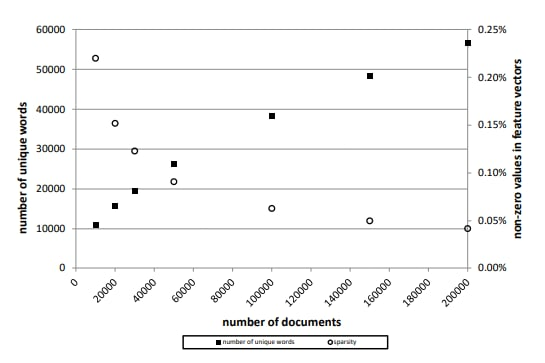
\includegraphics[width=\textwidth]{chapter/chapter1/figure1.1.jpg}
\caption{The graph represents a dependency between the number of documents and the number of unique words in a document collection.The documents represent customer reviews with the minimal, maximal, and average lengths equal to 1, 400, and 24 words.}
\end{figure}

\begin{itemize}
    \item For many tasks, there often exists a scarcity of labeled data. This is because the labeling process, usually performed manually, is very demanding. A special situation is that there are instances of positive training data for a specific problem, but negative examples are missing.

    \item In many situations, the distribution of the data in terms of classes or topics is not balanced. This means, that some classes have many more instances than the others which is generally a problem for learning. An example is the field of sentiment analysis, where the positive reviews in certain product categories are much more common than the negative ones.
\end{itemize}


\section{The Text Mining Process}
To find useful knowledge in a collection of text documents involves many different steps. To arrange them into a meaningful order, we might look at the general text mining process.It consists of the following steps \cite{ref271,ref133,ref196}:

\begin{itemize}
    \item \textbf{Defining the problem:} This step is actually independent of any actions which may subsequently be taken. Here, the problem domain needs to be understood and the questions to be answered, defined.
    
    \item \textbf{Collecting the necessary data:} The sources of texts containing the desired information need to be identified and the documents collected.The texts can come from within a company (internal database or archive) or from external sources, from the web, for example. In this case, web scrapers need to be frequently implemented to directly grab the content of the web pages.Alternatively, the API of some web based systems can be used to retrieve the data. After retrieval, texts are stored so they are ready for further analysis.
    
    \item \textbf{Defining features:} Features that well characterize the texts and are suitable for the given task need to be defined. The features are typically based on the content of the documents. A very simple approach, bag-of-words with binary attribute weighting, takes every word as a boolean feature. Its value indicates whether or not the word is in a document. Other methods might use more complicated weighting schemes or features that are derived from the words (modified words, combinations of words, etc.).
    
    \item \textbf{Analyzing the data:} This is the process of finding patterns in data. According to the type of task to be solved (e.g., classification), a specific model or algorithm is selected and its properties and parameters defined. Then, the model can be applied to the data so a solution to the solved problem can be found. To solve a specific problem, more models are usually available. The choice is not explicitly given in advance. The models have different characteristics that influence the data mining process and its result. The model can be (white box) or does not have to be (black box) well interpretable by a human. Some models have higher computational complexity than the others. According to the utilization of the model, fast creation can be preferred over fast application or vice versa. The suitability of a model is often strongly dependent on the data. The same model can provide excellent results for one data set while it can completely fail for another. Thus, selecting a proper model, finding the right structure for it, and tuning the parameters often requires a lot of experimental effort.
    
    \item \textbf{Interpreting the results:} Here, some results are obtained from the analysis. We need to carefully look at them and relate them to the problem we wanted to solve. This phase might include verification and validation steps in order to increase the reliability of the results.
\end{itemize}

\section{ Machine Learning for Text Mining}

\textit{Machine learning} \cite{ref199} as part of computer science and informatics is one of the most practically oriented areas of artificial intelligence \cite{ref161}. It was inspired by the ability to learn – in other words, to gain new or additional knowledge, which is one of important characteristics of living organisms. Machine learning as a
science focuses on looking for and developing algorithms, which can simulate or
emulate mental abilities of living organisms from the learning point of view.

Learned knowledge may not completely address everything – for it is something of a general nature – but, it allows us to solve future problems that did not
occur frequency, in the same form and/or environment in the past. If such a future problem is similar to something which has already occured, it is often not
possible to solve it using the exact instructions from the past; however, a similar
solution (or procedure) can hopefully be successful in most (or ideally, all) cases
that are yet to occur.

Machine learning is one of the modern tools that includes anything which can
be useful. Today, it consists of tens of various algorithms, and research constantly
brings modified or completely new algorithms, sometimes replacing the older
ones because the field of machine learning is strongly dominated by the practical
needs of the real world that are growing in time. In addition to algorithms and
relevant information technologies, machine learning inevitably uses mathematics, in particular the theory of probability, statistics, combinatorics, mathematical
analysis, and a set of other essential disciplines.

To solve problems with help of computers, machine learning differs from
the traditional method, which depends on applying carefully implemented and
debugged programs to input data. The traditional computer program consists of
sets of instructions that process the input data and provide the output using a set
of predefined parameters, which are provided externally. An example is a computer program that searches for a pre - set list of solutions to expected problems,
something like a table containing results for combinations of input values or
a set of mathematical equations. Such a program can be – in a simplified way–
considered as a function \textit{f(x) = y}, which for a given input x returns an output y,
however, provided that \textit{f(x)} is reliably known. Without knowing such a function,
it is necessary to estimate or approximate it.

If the needed conditions and rules are observed, the result is guaranteed because it is based on mathematically proved theorems and methods. Unfortunately, if there are–often even very small– changes in data or working environment, such a program is predisposed to a fundamental error or malfunction. For example, analyzed text data may begin to contain new terms that were not known when the program was created, or it becomes necessary to start analyzing such data in another language. In such a case, it is inevitable to rework, often completely, that program.

Machine learning can use an existing implemented algorithm, retrain it with
other examples and apply such new or extended knowledge to solving a new
problem. A certain defect might be that this knowledge is not supported enough
by mathematical proofs – in machine learning, the support comes from empirical
proofs and heuristics. \\

\begin{figure}[H]
    \centering
    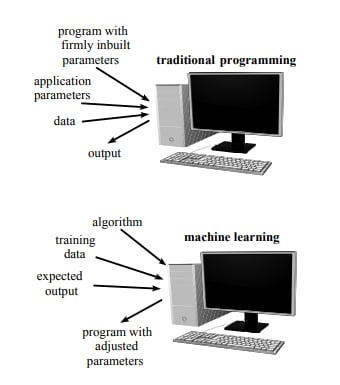
\includegraphics[width = 0.7\textwidth]{chapter/chapter1/figure1.2.jpg}
    \caption{ Traditional programming versus machine learning – illustration of the principles.}
\end{figure}

A simple illustration of the difference between traditional methods and machine learning is shown in Figure 1.2.

Determining the structure of models and their parameters is the goal of the
\textit{training} process, which uses (often iteratively) the presented training samples for
this purpose.The success rate of the training phase must be measured by \textit{testing},
which uses another set of samples which are not part of the training process.

\subsection{ Inductive Machine Learning}

Current methods, oriented on solving practical problems for example \cite{ref221,ref208,ref75}, are particularly based on inductive approaches.The inductive learning is based on the generalization of (many) specific samples for a given problem area. The samples are comprised of collected \textit{data}. For purpose of this book, that part of data, which is relevant for solving a given problem, is called \textit{information}.Then, generalized information forms \textit{knowledge}.The main task of machine learning is mining knowledge hidden in large collections of data.

Having a set of n samples of data items, $\{x_1, x_2, \dots, x_n\}$, and knowing for
each sample  $x_i$
its correct result $y_i$
, the approximate function $\hat{f}(x) \approx f(x)$. The
accuracy of such approximation depends naturally on the quality of samples –
how well they can cover (or represent) all possible data items. In the real world,
typically, not all possible data items are available for a given moment, or there might be so high (whether final or infinite) a number of such items that it is
practically impossible to process them within an available time period. At the
very least, data that may occur in the future may not be known now and moreover,
may not be fully represented by familiar data from the past.

Unlike the traditional applications of computer programs, machine learning
aims at automatically discovering the appropriate parameters of a selected algorithm, the implementation of which may already be available, but which needs
its parameters adjusted to specific data.

\section{Three Fundamental Learning Directions}

Depending on information provided by collected teaching samples, the current
machine learning sphere distinguishes three fundamental directions:

\begin{itemize}
    \item Supervised learning
    \item Unsupervised learning
    \item Semi-supervised learning
\end{itemize}

\subsection{ Supervised Machine Learning}

Known also as learning with a teacher, supervised machine learning relies on
labeled training samples. Each sample $x_i$ has its corresponding function value $y_i$:

\begin{equation*}
    y_i = f(x_i)
\end{equation*}

If the function $y_i$ is defined as non-numerical, its values are labels of classes.
For example, books may be classified according to verbal evaluation by their
readers who also assign a decision (label) $y_i \in \{\text{\textit{interesting}}, \text{\textit{tedious}}, \text{\textit{neutral}}\}$.
A classification algorithm learns using the labeled samples. This learning process
is called \emph{learning with a teacher} because the trained algorithm has feedback
based on the knowledge of the correct answers (labels). The feedback is provided
by the ‘teacher’ that supervises the correctness of classifications and the ‘learner’
knows whether its answer was right or not so that it can improve its knowledge —
appropriately adjusted parameters of the algorithm.

The regression methods for numeric functions are not discussed because they
are not relevant here.

\subsection{Unsupervised Machine Learning}
Unlike supervised machine learning, the unsupervised version misses feedback
from the absent teacher, thus the learners must learn themselves. The term ‘absent teacher’ means that the available training samples $x_i$
lack their appropriate class labels, therefore it is not directly possible to reveal what is relevant for each
class. In addition, it is not known what (and how many) classes exist for a given
case. The task is now not only to learn how to classify correctly but also to which
classes.

This branch of machine learning is called \emph{learning without a teacher} and employs various clustering algorithms and methods. Based on the contents of $x_i$’s,
the clustering algorithms try to detect which samples are similar enough to establish their particular cluster. Then, each cluster represents a class. Usually, it
is necessary to define (classes) in advance how many clusters should be generated; this is a frequent problem. Too few clusters can mean too vague knowledge mined from the data. The more clusters, the more specific each of them
is; however, too many clusters lack the property of being generalized knowledge
extracted from the samples – in the extreme case, each cluster contains only one
case, which is not very useful knowledge.

There exist also certain clustering algorithms that are able to discover the
number of convenient clusters; for example, the EM (expectation-maximization)
algorithm is worth mentioning. For more details, see \cite{ref112} chapter 8.5. 
EM assigns a probability distribution to each instance which indicates the probability of
its belonging to each of the clusters. EM can decide how many clusters to create
by cross-validation, or it can be specified \emph{a priori} how many clusters to generate.

The unsupervised learning belongs to more difficult and demanding learning
methods because it must work with less information. However, clustering today
constitutes one of the highly needed applications in the real world. An interested
reader can find more information concerning the clustering methods in \cite{ref142,ref230,ref22,ref254}, and many others.

\subsection{ Semi-supervised Machine Learning}

A modern machine learning branch is semi-supervised machine learning, which
– as its name suggests – represents something in between the extreme cases of supervised and unsupervised learning methods. In semi-supervised machine learning, the learner is given only a few labeled training samples and many unlabeled
ones.

The labeled samples provide some valuable initial information, which makes
it easier to separate (and label) unlabeled training samples so that the correct
classes can be generated.

This task is typical for contemporary situations when it is relatively much
easier to automatically collect and store a lot of unlabeled data than to laboriously
label them all.

As a result of the use of modern information and communication technologies
(the Internet, social networks), while there is an increasing amount of generally
valuable (and not only) textual data on a daily basis their processing, for example from a semantic point of view, is now completely beyond human ‘manual’
processing and research.

A limited number of training samples gives a limited amount of information
which can, however, be used advantageously for advanced text analysis. In any
case, this limited information provides some guidance on how to deal with incomplete (unlabeled) data items. A teacher can prepare a small set of samples
with answers (classification results), which may be used by the learner as a kind
of clue to help solve the class assignment with respect to non-classified training
items. At the same time, it makes it possible to better determine the number and
types of suitable classification classes.

A good introduction with examples of several algorithms (Self-training, Cotraining, and some others) can be found in \cite{ref1}.

\section{Big Data}

One of the problems that we can experience in text mining is that there are too
many data examples available. On the one hand, it can be considered positive
in terms of sufficient coverage of data with training examples. However, on the
other hand, it usually leads to great difficulties due to too high computational
complexity (time and memory), which the available hardware may not be able to
handle. This is a problem known as \textit{Big Data} (which is, however, not discussed
in this book; as an introduction, a reader may refer to, for example, \cite{ref147,ref152}).

For text mining, the mentioned big-data problem is often characteristic. The
reason is that, thanks to broadly available world-wide web technologies like the
Internet, textual data accumulate incredibly fast every day. Various social networks belong to most generous data providers and in principle, they represent
a very valuable source of information not only for the contributors. Unfortunately, it is not known how to define a mathematical function, which would be
able to process that natural-language based textual data so that the data may be
properly analyzed from its semantic point of view like human researchers can.
Because of the huge amount of the data, it is necessary to use informatics and
computers, which is where machine learning helps.

\section{About this book}

Today, a lot of good publications and books are already available for familiarization with machine learning, for example \cite{ref199, ref152, ref187, ref261}. Tens of books
from various publishers deal with many different problem areas from the machine learning point of view, and a reader will, undoubtedly be able to find what
her or his specific interests need. Our goal is, therefore, not to teach machine learning in general. Instead, we would like to show how machine learning can be
used to solve practical tasks in a specific domain, which is text data analysis.

In order to obtain some real results and enable readers to implement some
of the described procedures, we decided to use the R programming language.
R is a great statistical software package with many advantages. It is free, it is
interpreted (the same code can be run on many platforms), and provides an extensive functionality contained in many available packages. It is used by many
researchers and practitioners all over the world. The solutions of problems using
R are, however, often not suitable for large scale problems because R works only
with data that fit to the memory of a computer and is often slow (the reduced
speed is also because it is very flexible through dynamic typing).

In R and its available libraries, many machine learning algorithms are already
implemented. It is, therefore, necessary to provide them with prepared data in
a desired format, get the results, and display, visualize, or evaluate them. All
these steps are combined in computer programs (scripts) that are run on an R
interpreter.

In individual chapters dealing with typical text mining tasks, the code that
is used to demonstrate the algorithms and solve some practical problems is also
presented. To enable readers to understand the code, some of the R basics are
included in the book too. We do not try to explain all aspects of the language,
all available algorithm implementations, their possible parameters, inputs, and
outputs, but only what is necessary for our specific examples. All other details
can always be found in the newest description (manual) of the used R package.
